% Streaming Semi-CRF Algorithm Supplement
% For inclusion in manuscript supplemental material
%
% Required packages:
% \usepackage[ruled,vlined,linesnumbered]{algorithm2e}
% \usepackage{amsmath,amssymb}

\documentclass{article}
\usepackage[T1]{fontenc}
\usepackage[margin=1.25in]{geometry}  % Increased margins
\usepackage[ruled,vlined,linesnumbered]{algorithm2e}
\usepackage{amsmath,amssymb}
\usepackage{xcolor}
\usepackage{hyperref}
\usepackage{tikz}
\usepackage{float}
\usetikzlibrary{arrows.meta,positioning,patterns,decorations.pathreplacing,calc}

\begin{document}

\section*{Supplemental Material: Streaming Semi-CRF Inference}

This supplement provides formal algorithmic details for the streaming Semi-CRF implementation.

%==============================================================================
\section{Notation}
%==============================================================================

\begin{table}[h]
\centering
\begin{tabular}{c l l}
\hline
\textbf{Symbol} & \textbf{Description} & \textbf{Shape} \\
\hline
$T$ & Padded sequence length (batch dimension) & scalar \\
$L_b$ & True (unpadded) length for batch element $b$ & scalar \\
$K$ & Maximum segment duration & scalar \\
$C$ & Number of labels (states) & scalar \\
$C_{\text{PAD}}$ & Padded label count (next power of 2) & scalar \\
$B$ & Batch size & scalar \\
$\mathcal{S}_{t,c}$ & Cumulative centered scores & $(B, T+1, C)$ \\
$f_\theta(t,c)$ & Raw projected encoder emissions & $(B, T, C)$ \\
$\nu_{b,c}$ & Sequence-level emission baseline (Eq.~\ref{eq:baseline}) & $(B, C)$ \\
$\bar{f}_\theta(t,c)$ & Centered emissions: $f_\theta(t,c) - \nu_{b,c}$ & $(B, T, C)$ \\
$\mathcal{T}_{c',c}$ & Transition scores (source $c'$ to dest $c$) & $(C, C)$ \\
$\mathcal{B}_{k,c}$ & Duration bias for duration $k$, label $c$ & $(K, C)$ \\
$\mathcal{P}^{\text{start}}_{t,c}$ & Start boundary projection (optional) & $(B, T, C)$ \\
$\mathcal{P}^{\text{end}}_{t,c}$ & End boundary projection (optional) & $(B, T, C)$ \\
$\tilde{\alpha}_t(c)$ & Log-forward message at position $t$, label $c$ & $(B, C)$ \\
$\tilde{\beta}_t(c)$ & Log-backward message & $(B, C)$ \\
$\boldsymbol{\alpha}$ & Forward ring buffer & $(B, K, C)$ \\
$\boldsymbol{\beta}$ & Backward ring buffer & $(B, 2K, C)$ \\
$\Omega$ & Checkpointed ring buffer states & $(B, N, K, C)$ \\
$\mathcal{N}$ & Cumulative log-normalization factors & $(B, N)$ \\
$\Delta$ & Checkpoint interval ($\approx \sqrt{TK}$) & scalar \\
$\tau$ & Tile size for label dimension & scalar \\
$\log Z$ & Log partition function & $(B,)$ \\
\hline
\end{tabular}
\caption{Notation. Tilde ($\tilde{\cdot}$) denotes log-domain quantities. $N = \lceil T / \Delta \rceil$ is the number of checkpoints.}
\label{tab:notation}
\end{table}

\textbf{Indexing conventions.}
Positions $t \in \{0, \ldots, T\}$ index \emph{boundaries} between tokens; cumulative scores $\mathcal{S}_{t,c}$ are defined at boundaries, with $\mathcal{S}_{0,c} = 0$.
Emissions $f_\theta(t, c)$ are defined at tokens $t \in \{0, \ldots, T{-}1\}$ (0-indexed).
Segments are half-open intervals $[s, s{+}k)$ covering tokens $s, s{+}1, \ldots, s{+}k{-}1$, so that the content score is $\mathcal{S}_{s+k, c} - \mathcal{S}_{s, c}$.
Durations are 1-indexed: $k \in \{1, \ldots, K\}$, stored at 0-indexed positions $k{-}1$ in code.

%==============================================================================
\section{Edge Potential Decomposition}
%==============================================================================

The key innovation enabling $O(KC)$ memory is computing edge potentials on-the-fly from cumulative scores. We first describe the construction of these cumulative scores, then the edge potential formula.

\subsection{Emission Baseline Centering}
\label{sec:emission_baseline}

Let $f_\theta(t, c)$ denote the raw projected encoder emissions at token $t$ for label $c$. We introduce \emph{globally-centered emissions}, a formulation that couples local segment scores to global label statistics via a per-label, per-sequence baseline subtraction. While primarily motivated by numerical stability at $T > 10^5$, this formulation induces an implicit adaptive duration prior (Section~\ref{sec:centering_semantics}) that we find beneficial for segmentation stability in label-imbalanced sequences.

Before constructing the prefix sums, we subtract the \emph{sequence-level emission baseline}:
\begin{equation}
\label{eq:baseline}
\nu_{b,c} = \frac{1}{T} \sum_{u=0}^{T-1} f_\theta(u, c), \qquad
\bar{f}_\theta(t, c) = f_\theta(t, c) - \nu_{b,c}
\end{equation}

\noindent where $T$ is the padded sequence length.\footnote{The implementation computes the baseline over the full (padded) sequence via \texttt{scores\_float.mean(dim=1, keepdim=True)}.  Although tokens $u \ge L_b$ are masked in the DP (no segment may include them), they still influence $\nu_{b,c}$ and thus shift the centered emissions at all valid positions $u < L_b$.  The effective model therefore depends on the padding emissions and the padded length $T$, not only on the true sequence.  This definition is well-defined only relative to a fixed padding scheme (fixed $T$ and fixed padding-token semantics).  For the primary use case of fixed-length genomic windows, $L_b = T$ for all batch elements and the distinction vanishes.  A masked-mean variant ($\nu_{b,c} = L_b^{-1}\sum_{u=0}^{L_b-1} f_\theta(u,c)$) would eliminate the padding dependence for heterogeneous batch lengths.}
Globally-centered emissions are part of the model definition; all reported results use this formulation unless otherwise stated.

\noindent For each batch element $b$, the cumulative scores are then defined over the centered emissions:
\begin{equation}
\label{eq:cumscores}
\mathcal{S}_{0, c} = 0, \qquad \mathcal{S}_{t, c} = \sum_{u=0}^{t-1} \bar{f}_\theta(u, c)
\end{equation}

\noindent so that the content score for a segment $[s, s+k)$ labeled $c$ becomes
\begin{equation}
\label{eq:content_centered}
\mathcal{S}_{s+k, c} - \mathcal{S}_{s, c}
= \sum_{u=s}^{s+k-1} f_\theta(u, c) \;-\; \nu_{b,c} \cdot k
\end{equation}

\noindent Equation~\eqref{eq:content_centered} shows that centering introduces a data-dependent term $-\nu_{b,c} \cdot k$ that couples label identity to segment duration. Equivalently, the effective duration model for label $c$ is $\mathcal{B}_{k,c} - \nu_{b,c} \cdot k$, where the second term is an \emph{adaptive duration prior} derived from the sequence-level emission statistics (Section~\ref{sec:centering_semantics}).

\subsection{Edge Potentials}

The edge potential for a segment ending at position $t$ with duration $k$, transitioning from source label $c'$ to destination label $c$, is:

\begin{equation}
\label{eq:streaming_potential}
\tilde{\psi}(t, k, c, c') =
\underbrace{\left(\mathcal{S}_{t, c} - \mathcal{S}_{t-k, c}\right)}_{\text{centered content}} +
\underbrace{\mathcal{B}_{k, c}}_{\text{duration bias}} +
\underbrace{\mathcal{T}_{c', c}}_{\text{transition}}
+ \underbrace{\mathcal{P}^{\text{start}}_{t-k, c} + \mathcal{P}^{\text{end}}_{t-1, c}}_{\text{boundary (optional)}}
\end{equation}

\noindent where $k \in \{1, \ldots, K\}$ is the duration, $c$ is the destination state, and $c'$ is the source state. The optional boundary projections $\mathcal{P}^{\text{start}}$ and $\mathcal{P}^{\text{end}}$ score segment start/end positions (e.g., for detecting boundary-specific features). The prefix-sum decomposition allows $O(1)$-in-$k$ edge computation (constant-time in the duration) instead of $O(k)$ accumulation.

%==============================================================================
\section{Streaming Forward Algorithm}
%==============================================================================

Algorithm~\ref{alg:streaming_forward} maintains a ring buffer $\boldsymbol{\alpha} \in \mathbb{R}^{K \times C}$ storing the $K$ most recent forward messages (Figure~\ref{fig:memory_layout}a). Following the Flash Attention~\cite{dao2022flashattention} and Mamba~\cite{gu2023mamba} pattern, we normalize at checkpoint boundaries to prevent scale drift and maintain numerical stability at extreme $T$.

\begin{algorithm}[t]
\caption{Streaming Semi-CRF Forward Scan}\label{alg:streaming_forward}
\KwIn{$\mathcal{S}$, $\mathcal{T}$, $\mathcal{B}$, checkpoint interval $\Delta$}
\KwOut{$\log Z$, checkpoints $(\Omega, \mathcal{N})$}
\BlankLine
$\boldsymbol{\alpha} \gets -\infty$; \quad $\boldsymbol{\alpha}[0, :] \gets 0$; \quad $\mathcal{N}_{\text{accum}} \gets 0$\;
$\Omega[0] \gets \boldsymbol{\alpha}$; \quad $\mathcal{N}[0] \gets 0$\;
\BlankLine
\For{$t \gets 1$ \KwTo $T$}{
    $\mathbf{v}_t \gets -\infty \in \mathbb{R}^C$\;
    \For{$k \gets 1$ \KwTo $\min(K, t)$}{
        $\tilde{\boldsymbol{\alpha}}_{\text{prev}} \gets \boldsymbol{\alpha}[(t-k) \bmod K, :]$\;
        $\mathbf{h} \gets \bigl(\mathcal{S}_{t,:} - \mathcal{S}_{t-k,:}\bigr) + \mathcal{B}_{k,:}$\;
        $\mathbf{E} \gets \mathbf{h}[:, \text{None}] + \mathcal{T}^\top$\;
        $\mathbf{s}_k \gets \text{LSE}(\tilde{\boldsymbol{\alpha}}_{\text{prev}}[\text{None}, :] + \mathbf{E}, \text{axis}=1)$\;
        $\mathbf{v}_t \gets \text{LSE}(\mathbf{v}_t, \mathbf{s}_k)$\;
    }
    $\boldsymbol{\alpha}[t \bmod K, :] \gets \mathbf{v}_t$\;
    \BlankLine
    \If(\tcp*[f]{Normalize at checkpoint~\cite{dao2022flashattention}}){$t \bmod \Delta = 0$}{
        $n \gets t / \Delta$\;
        \tcp{Only normalize active sequences ($t \le L_b$) to avoid phantom shifts}
        $s_b \gets \begin{cases} \max_c \mathbf{v}_{t,b}(c) & \text{if } t \le L_b \\ 0 & \text{otherwise} \end{cases}$\;
        $\mathcal{N}_{\text{accum}} \gets \mathcal{N}_{\text{accum}} + s_b$; \quad $\boldsymbol{\alpha} \gets \boldsymbol{\alpha} - s_b$\;
        $\Omega[n] \gets \boldsymbol{\alpha}$; \quad $\mathcal{N}[n] \gets \mathcal{N}_{\text{accum}}$\;
    }
}
\BlankLine
$\log Z \gets \text{LSE}(\boldsymbol{\alpha}[T \bmod K, :]) + \mathcal{N}_{\text{accum}}$\;
\Return{$\log Z$, $(\Omega, \mathcal{N})$}\;
\end{algorithm}

\textbf{Memory}: $O(KC)$ ring buffer + $O(\sqrt{T/K} \cdot KC)$ checkpoints. \textbf{Time}: $O(TKC^2)$.

\begin{figure}[t]
\centering
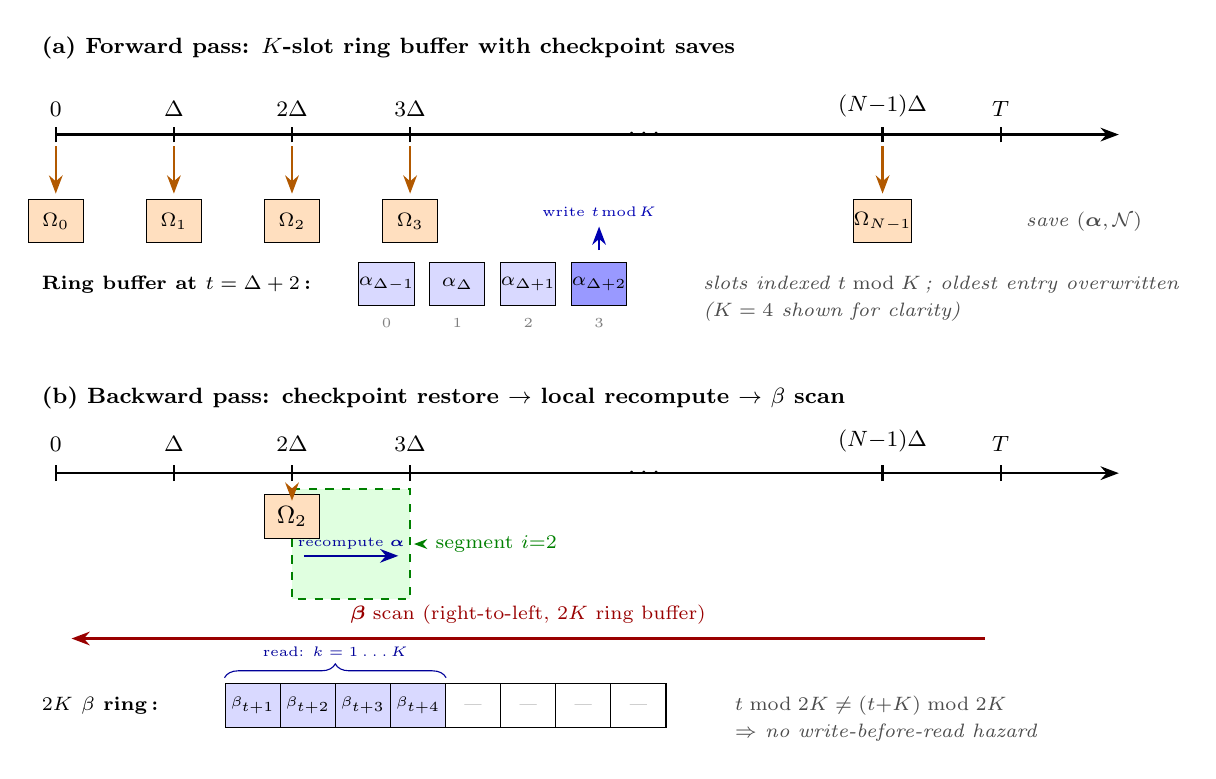
\begin{tikzpicture}[
    >=Stealth,
    slot/.style={draw, minimum width=0.7cm, minimum height=0.55cm, inner sep=0pt, font=\scriptsize},
    slotactive/.style={slot, fill=blue!15},
    slotwrite/.style={slot, fill=blue!40},
    slotold/.style={slot, fill=gray!15},
    ckpt/.style={draw, fill=orange!25, minimum width=0.7cm, minimum height=0.55cm, inner sep=0pt, font=\scriptsize},
    timeline/.style={draw, thick, ->},
    brace/.style={decorate, decoration={brace, amplitude=5pt, raise=2pt}},
    bracebelow/.style={decorate, decoration={brace, amplitude=5pt, raise=2pt, mirror}},
    lbl/.style={font=\footnotesize},
    sublbl/.style={font=\scriptsize\itshape, text=black!70},
]

% ========== Panel (a): Forward Pass ==========
\node[font=\footnotesize\bfseries, anchor=west] at (-0.3, 2.9) {(a) Forward pass: $K$-slot ring buffer with checkpoint saves};

% Timeline
\draw[timeline] (0, 1.8) -- (13.5, 1.8);
\foreach \x/\lab in {0/0, 1.5/$\Delta$, 3/$2\Delta$, 4.5/$3\Delta$, 10.5/$(N{-}1)\Delta$, 12/$T$} {
    \draw[thick] (\x, 1.7) -- (\x, 1.9);
    \node[lbl, above] at (\x, 1.9) {\lab};
}
% Dots for gap
\node at (7.5, 1.8) {$\cdots$};

% Checkpoint saves (arrows down)
\foreach \x/\n in {0/0, 1.5/1, 3/2, 4.5/3, 10.5/{N{-}1}} {
    \draw[->, orange!70!black, thick] (\x, 1.65) -- (\x, 1.05);
    \node[ckpt] at (\x, 0.7) {$\Omega_{\n}$};
}
\node[sublbl, anchor=west] at (12.2, 0.7) {save $(\boldsymbol{\alpha}, \mathcal{N})$};

% Ring buffer detail: show state at t within segment [Δ, 2Δ)
% Ring buffer box
\node[font=\scriptsize\bfseries, anchor=west] at (-0.3, -0.1) {Ring buffer at $t = \Delta + 2$\,:};
\foreach \i/\lab/\sty in {0/$\alpha_{\Delta-1}$/slotactive, 1/$\alpha_{\Delta}$/slotactive, 2/$\alpha_{\Delta+1}$/slotactive, 3/{$\alpha_{\Delta+2}$}/slotwrite} {
    \node[\sty] (ring\i) at ({4.2 + \i*0.9}, -0.1) {\lab};
}
% slot labels below
\foreach \i in {0,...,3} {
    \node[font=\tiny, text=black!50, below=1pt] at (ring\i.south) {$\i$};
}
% Write arrow
\draw[->, blue!70!black, thick] (ring3.north) ++(0, 0.15) -- ++(0, 0.3) node[above, font=\tiny, blue!70!black] {write $t\!\bmod\!K$};
% mod K label
\node[sublbl, anchor=west] at (8.1, -0.1) {slots indexed $t \bmod K$\,; oldest entry overwritten};
\node[sublbl, anchor=west] at (8.1, -0.45) {($K = 4$ shown for clarity)};

% ========== Panel (b): Backward Pass ==========
\node[font=\footnotesize\bfseries, anchor=west] at (-0.3, -1.55) {(b) Backward pass: checkpoint restore $\to$ local recompute $\to$ $\beta$ scan};

% Timeline
\draw[timeline] (0, -2.5) -- (13.5, -2.5);
\foreach \x/\lab in {0/0, 1.5/$\Delta$, 3/$2\Delta$, 4.5/$3\Delta$, 10.5/$(N{-}1)\Delta$, 12/$T$} {
    \draw[thick] (\x, -2.6) -- (\x, -2.4);
    \node[lbl, above] at (\x, -2.35) {\lab};
}
\node at (7.5, -2.5) {$\cdots$};

% Highlight active segment [2Δ, 3Δ)
\fill[green!12] (3, -2.7) rectangle (4.5, -4.1);
\draw[green!50!black, thick, dashed] (3, -2.7) rectangle (4.5, -4.1);

% Restore arrow from checkpoint into segment
\node[ckpt] at (3.0, -3.05) {\small$\Omega_2$};
\draw[->, orange!70!black, thick] (3.0, -2.75) -- (3.0, -2.85);

% Forward recompute arrow within segment
\draw[->, blue!60!black, thick] (3.15, -3.55) -- (4.35, -3.55);
\node[font=\tiny, blue!60!black] at (3.75, -3.4) {recompute $\boldsymbol{\alpha}$};

% Segment label to the right of the box
\node[font=\scriptsize, green!50!black, anchor=west] at (4.7, -3.4) {segment $i{=}2$};
\draw[->, green!50!black, thin] (4.65, -3.4) -- (4.55, -3.4);

% Beta scan arrow (right to left) below the segment boxes
\draw[<-, red!60!black, thick] (0.2, -4.6) -- (11.8, -4.6);
\node[font=\scriptsize, red!60!black, above] at (6, -4.55) {$\boldsymbol{\beta}$ scan (right-to-left, $2K$ ring buffer)};

% Beta ring buffer detail
\node[font=\scriptsize\bfseries, anchor=west] at (-0.3, -5.45) {$2K$ $\beta$ ring\,:};
\foreach \i/\sty in {0/slotactive, 1/slotactive, 2/slotactive, 3/slotactive, 4/slot, 5/slot, 6/slot, 7/slot} {
    \node[\sty] (bring\i) at ({2.5 + \i*0.7}, -5.45) {};
}
% Labels for slots
\node[font=\tiny] at (bring0) {$\beta_{t+1}$};
\node[font=\tiny] at (bring1) {$\beta_{t+2}$};
\node[font=\tiny] at (bring2) {$\beta_{t+3}$};
\node[font=\tiny] at (bring3) {$\beta_{t+4}$};
\node[font=\tiny, text=black!40] at (bring4) {---};
\node[font=\tiny, text=black!40] at (bring5) {---};
\node[font=\tiny, text=black!40] at (bring6) {---};
\node[font=\tiny, text=black!40] at (bring7) {---};
% Brace over read slots
\draw[brace, blue!60!black] (bring0.north west) -- (bring3.north east) node[midway, above=6pt, font=\tiny, blue!60!black] {read: $k = 1 \ldots K$};
% No-conflict annotation
\node[sublbl, anchor=west] at (8.5, -5.45) {$t \bmod 2K \neq (t{+}K) \bmod 2K$};
\node[sublbl, anchor=west] at (8.5, -5.8) {$\Rightarrow$ no write-before-read hazard};

\end{tikzpicture}
\caption{Memory layout for streaming semi-CRF inference.
\textbf{(a)}~During the forward pass, the ring buffer cycles through $K$ slots via $t \bmod K$ indexing; at every $\Delta$-th position, the full ring buffer state $\Omega_i$ and cumulative log-normalizer $\mathcal{N}_i$ are checkpointed.
\textbf{(b)}~During the backward pass, each checkpoint segment is processed independently: $\boldsymbol{\alpha}$ is restored from $\Omega_i$ and recomputed locally (blue arrow), while $\boldsymbol{\beta}$ is scanned right-to-left through a $2K$-slot ring buffer that prevents the write-before-read hazard (Section~\ref{sec:2k_ring}). Total memory is $O(KC)$ for ring buffers $+$ $O(\sqrt{T/K} \cdot KC)$ for checkpoints, independent of sequence length $T$.}
\label{fig:memory_layout}
\end{figure}

%==============================================================================
\section{Backward Pass with Checkpointing}
%==============================================================================

Algorithm~\ref{alg:streaming_backward} processes segments in reverse, recomputing $\alpha$ from checkpoints following gradient checkpointing~\cite{chen2016training} (Figure~\ref{fig:memory_layout}b). The saved $\mathcal{N}_i$ restores the true scale when computing marginals.

\begin{algorithm}[t]
\caption{Streaming Semi-CRF Backward Pass}\label{alg:streaming_backward}
\KwIn{$\mathcal{S}$, $\mathcal{T}$, $\mathcal{B}$, checkpoints $(\Omega, \mathcal{N})$, $\log Z$, upstream $\partial \mathcal{L}/\partial Z$}
\KwOut{$\nabla \mathcal{S}$, $\nabla \mathcal{T}$, $\nabla \mathcal{B}$}
\BlankLine
$\boldsymbol{\beta} \gets -\infty \in \mathbb{R}^{2K \times C}$; \quad $\boldsymbol{\beta}[T \bmod 2K, :] \gets 0$\;
Initialize gradient accumulators\;
\BlankLine
\For{$i \gets N_{\text{ckpts}}-1$ \KwTo $0$}{
    $t_{\text{start}} \gets i \cdot \Delta$; \quad $t_{\text{end}} \gets \min((i+1) \cdot \Delta, T)$\;
    $\mathcal{N}_i \gets \mathcal{N}[i]$\;
    $\boldsymbol{\alpha}_{\text{local}} \gets$ \textsc{RecomputeAlpha}($\Omega[i]$, $t_{\text{start}}$, $t_{\text{end}}$)\;
    \BlankLine
    \For{$t \gets t_{\text{end}}-1$ \KwTo $t_{\text{start}}$}{
        $\tilde{\boldsymbol{\alpha}}_t \gets \boldsymbol{\alpha}_{\text{local}}[t - t_{\text{start}}, :]$\;
        $\tilde{\boldsymbol{\beta}}_t \gets -\infty$\;
        \BlankLine
        \For{$k \gets 1$ \KwTo $\min(K, T-t)$}{
            $\tilde{\boldsymbol{\beta}}_{\text{next}} \gets \boldsymbol{\beta}[(t+k) \bmod 2K, :]$\tcp*[r]{$2K$ ring buffer}
            $\tilde{\psi} \gets$ Eq.~\eqref{eq:streaming_potential}\;
            \BlankLine
            \tcp{Log-norm correction restores true $\alpha$ scale}
            $\log \mu \gets \tilde{\boldsymbol{\alpha}}_t[\text{None}, :] + \tilde{\psi} + \tilde{\boldsymbol{\beta}}_{\text{next}}[:, \text{None}] + \mathcal{N}_i - \log Z$\;
            $\mu \gets \exp(\log \mu)$\;
            \BlankLine
            Accumulate $\nabla \mathcal{S}$, $\nabla \mathcal{T}$, $\nabla \mathcal{B}$ from $\mu$\;
            $\tilde{\boldsymbol{\beta}}_t \gets \text{LSE}(\tilde{\boldsymbol{\beta}}_t, \text{LSE}(\tilde{\psi} + \tilde{\boldsymbol{\beta}}_{\text{next}}[:, \text{None}], \text{axis}=0))$\;
        }
        $\boldsymbol{\beta}[t \bmod 2K, :] \gets \tilde{\boldsymbol{\beta}}_t$\tcp*[r]{$2K$ ring buffer}
    }
}
\Return{$\nabla \mathcal{S}$, $\nabla \mathcal{T}$, $\nabla \mathcal{B}$}\;
\end{algorithm}

%==============================================================================
\section{$2K$ Beta Ring Buffer}
\label{sec:2k_ring}
%==============================================================================

While the forward pass uses a ring buffer of size $K$ (sufficient since we only look back $K$ positions), the backward pass requires a ring buffer of size $2K$. This asymmetry arises from the different access patterns:

\textbf{Forward pass access pattern.} At position $t$, we read $\alpha$ values from positions $\{t-K, t-K+1, \ldots, t-1\}$---exactly $K$ previous positions. A ring buffer indexed by $t \bmod K$ suffices.

\textbf{Backward pass access pattern.} At position $t$, we read $\beta$ values from positions $\{t+1, t+2, \ldots, t+K\}$---$K$ future positions. However, we also write $\beta[t]$ while potentially still reading $\beta[t+K]$. If we used a ring buffer of size $K$, we would have:
\begin{align}
\text{write index:} \quad & t \bmod K \\
\text{read index for } k=K: \quad & (t+K) \bmod K = t \bmod K
\end{align}

This creates a \textbf{write-before-read hazard}: we would overwrite $\beta[t+K]$ before reading it. The $2K$ ring buffer eliminates this conflict:
\begin{equation}
t \bmod 2K \neq (t+K) \bmod 2K \quad \text{for all } t \geq 0
\end{equation}

\textbf{Memory cost.} The additional $KC$ floats is negligible compared to the $O(\sqrt{T/K} \cdot KC)$ checkpoint storage.

%==============================================================================
\section{Adaptive Loop Tiling}
\label{sec:tiling}
%==============================================================================

The marginal computation requires a $(C_{\text{PAD}} \times C_{\text{PAD}})$ matrix per $(t, k)$ pair, which at $C_{\text{PAD}}=64$ demands approximately 384 registers per thread. With 4+ warps, this exceeds available registers and causes spilling to slow local memory.

\textbf{Tiled computation.} We process the destination label dimension $c_{\text{dst}}$ in tiles of size $\tau$ (TILE\_C):
\begin{enumerate}
\item Load a $(\tau \times C_{\text{PAD}})$ tile of the marginal matrix
\item Accumulate gradients from the tile
\item Use online logsumexp for $\beta$ update across tiles (Flash Attention pattern~\cite{dao2022flashattention})
\end{enumerate}

This reduces peak register demand to approximately 120 per thread, enabling 4--8 warps without spilling.

\textbf{Adaptive tile sizing.} The tile size $\tau$ is selected based on $C$ to balance compile time, register pressure, and iteration count:

\begin{table}[h]
\centering
\begin{tabular}{c c c l}
\hline
$C_{\text{PAD}}$ & $\tau$ & Iterations & Rationale \\
\hline
$\leq 8$ & 4 & 2 & Minimal iteration count \\
$\leq 16$ & 8 & 2 & Minimal iteration count \\
$32$ & 16 & 2 & Balanced \\
$64$ & 16 & 4 & Moderate register pressure \\
$\geq 128$ & 32 & $\leq 8$ & Bounded compile time \\
\hline
\end{tabular}
\caption{Adaptive tile size selection via \texttt{\_compute\_tile\_c()}. The algorithm bounds iteration count to $\leq 8$ even at $C=256$ while keeping register pressure manageable.}
\label{tab:tile_sizing}
\end{table}

\textbf{Online logsumexp for $\beta$.} Since $\beta$ reduction spans multiple tiles, we use the Flash Attention online pattern:
\begin{align}
m^{(i)} &= \max(m^{(i-1)}, m_{\text{tile}}^{(i)}) \\
\ell^{(i)} &= \ell^{(i-1)} \cdot e^{m^{(i-1)} - m^{(i)}} + \sum_j e^{x_j^{(i)} - m^{(i)}}
\end{align}
where $m$ tracks the running maximum and $\ell$ tracks the running sum of exponentials, rescaled at each tile boundary.

%==============================================================================
\section{Reduced Atomics Strategy}
\label{sec:reduced_atomics}
%==============================================================================

GPU atomic operations are expensive and introduce non-determinism due to floating-point non-associativity. We employ three strategies to minimize their use:

\subsection{Local Accumulation for Per-Position Gradients}

For $\nabla \mathcal{S}_{t,c}$, the negative contribution (from segments starting at $t$) is the same position for all $k$ values. Instead of $K \times \text{tiles}$ atomic operations, we accumulate locally:

\begin{algorithm}[H]
\caption{Local Accumulation for $\nabla \mathcal{S}_t$}\label{alg:local_accum}
$\texttt{grad\_cs\_t\_local} \gets \mathbf{0} \in \mathbb{R}^{C_{\text{PAD}}}$\;
\For{$k \gets 1$ \KwTo $K$}{
    \For{\text{each tile}}{
        $\texttt{grad\_cs\_t\_local} \mathrel{-}= \sum_{c'} \mu_{\text{tile}}(t, k, c, c')$\tcp*[r]{Register accumulation}
    }
}
$\texttt{atomic\_add}(\nabla \mathcal{S}_t, \texttt{grad\_cs\_t\_local})$\tcp*[r]{Single write}
\end{algorithm}

\textbf{Speedup}: $K \times \text{tiles} \to 1$ atomic per position (e.g., $1000 \times 4 = 4000 \to 1$ at $K=1000$, $C=64$).

\subsection{Per-Duration Accumulation for Duration Bias}

For $\nabla \mathcal{B}_{k,c}$, we accumulate across all tiles for each $k$, then write once:

\begin{algorithm}[H]
\caption{Per-Duration Accumulation for $\nabla \mathcal{B}_k$}
\For{$k \gets 1$ \KwTo $K$}{
    $\texttt{grad\_db\_k\_local} \gets \mathbf{0} \in \mathbb{R}^{C_{\text{PAD}}}$\;
    \For{\text{each tile}}{
        $\texttt{grad\_db\_k\_local} \mathrel{+}= \sum_{c'} \mu_{\text{tile}}(t, k, c, c')$\;
    }
    $\texttt{atomic\_add}(\nabla \mathcal{B}_k, \texttt{grad\_db\_k\_local})$\tcp*[r]{Once per $k$}
}
\end{algorithm}

\textbf{Speedup}: $\text{tiles} \to 1$ atomic per $(t, k)$ pair.

\subsection{Segment-Isolated Workspace Buffers}

For shared parameters ($\nabla \mathcal{T}$, $\nabla \mathcal{B}$), cross-segment atomic contention introduces non-determinism. We allocate per-segment workspace buffers:

\begin{equation}
\texttt{grad\_tr\_workspace} \in \mathbb{R}^{B \times N_{\text{segments}} \times C_{\text{PAD}} \times C_{\text{PAD}}}
\end{equation}

\noindent (Padded to $C_{\text{PAD}}$ to prevent out-of-bounds access from masked Triton threads; sliced back to $C$ before reduction.)

Each checkpoint segment writes to its own slice, eliminating inter-segment atomics. The final reduction uses deterministic host-side operations:

\begin{align}
\nabla \mathcal{T}_{c',c} &= \texttt{einsum}(\text{``bsij, b} \to \text{ij''}, \texttt{workspace.sum(dim=1)}, \nabla_{\text{out}}) \\
\nabla \mathcal{B}_{k,c} &= \texttt{einsum}(\text{``bskc, b} \to \text{kc''}, \texttt{workspace.sum(dim=1)}, \nabla_{\text{out}})
\end{align}

\textbf{Determinism}: The segment-wise sum is deterministic (fixed order), and \texttt{einsum} performs a single reduction pass.

\textbf{Memory cost}: $O(B \cdot N_{\text{segments}} \cdot K \cdot C^2)$ workspace, which is acceptable since $N_{\text{segments}} \approx \sqrt{T/K}$ is typically small (e.g., 10--100 for $T=100\text{k}$, $K=1000$).

%==============================================================================
\section{Gradient Computation}
\label{sec:gradients}
%==============================================================================

Gradients are computed via marginal probabilities:

\begin{equation}
\mu(t, k, c, c') = \exp\bigl(\tilde{\alpha}_{t-k}(c') + \tilde{\psi}(t, k, c, c') + \tilde{\beta}_t(c) + \mathcal{N}_i - \log Z\bigr)
\end{equation}

For per-sequence parameters:
\begin{equation}
\nabla \mathcal{S}_{t,c} = \frac{\partial \mathcal{L}}{\partial Z_b} \cdot \left( \sum_{k, c'} \mu_b(t, k, c, c') - \sum_{k, c'} \mu_b(t+k, k, c, c') \right)
\end{equation}

For shared parameters, we accumulate per-batch then reduce via einsum:
\begin{align}
\nabla \mathcal{T}_{c',c} &= \sum_{b} \left( \frac{\partial \mathcal{L}}{\partial Z_b} \cdot \sum_{t,k} \mu_b(t, k, c, c') \right) \\
\nabla \mathcal{B}_{k,c} &= \sum_{b} \left( \frac{\partial \mathcal{L}}{\partial Z_b} \cdot \sum_{t, c'} \mu_b(t, k, c, c') \right)
\end{align}

\noindent The parentheses emphasize that each batch element's marginals are weighted by its upstream gradient \emph{before} summing across batches. This distinction matters when $\partial \mathcal{L}/\partial Z_b$ varies (e.g., masked sequences or weighted losses).

%==============================================================================
\section{Numerical Stability}
%==============================================================================

\subsection{Globally-Centered Emissions: Semantics and Motivation}
\label{sec:centering_semantics}

Globally-centered emissions (Eq.~\ref{eq:baseline}) serve dual purposes: numerical stabilization of the prefix sums, and adaptive regularization of the duration model.

\textbf{Numerical role.}
Without centering, cumulative scores grow as $\mathcal{S}_{T,c} = O(T)$ when encoder emissions have nonzero per-label means.  At genomic scale ($T > 100{,}000$), segment scores $\mathcal{S}_{t+k, c} - \mathcal{S}_{t, c}$ risk catastrophic cancellation---both operands reach magnitude $O(T)$ while their difference is $O(1)$.
Subtracting the per-label mean before accumulation reduces this to a zero-mean random walk whose cumulative sums have standard deviation $O(\sqrt{T})$ by the central limit theorem, analogous to how the log-sum-exp identity prevents overflow in softmax computation.
The current implementation uses float64 for the forward-backward recurrence, which tolerates large input magnitudes; centering provides additional insurance, ensuring that a future migration to float32 kernels would not require algorithmic changes.

\textbf{Modeling role.}
Global centering is \emph{not} a path-invariant transformation: subtracting a label-specific constant $\nu_{b,c}$ shifts segment scores by $-\nu_{b,c} \cdot k$, which is label-dependent and length-dependent.
A path-invariant centering (e.g., subtracting a per-position scalar $b_t = \max_c f_\theta(t,c)$ shared across labels) would cancel in the partition function because every valid segmentation covers each position exactly once.
Per-label centering does not cancel because different segmentations assign different labels to different positions, and $\nu_{b,c}$ varies across labels.

Concretely, the effective segment score under centering (Eq.~\ref{eq:content_centered}) is:
\begin{equation}
\label{eq:effective_score}
S_{\text{eff}}(c, s, k) = \sum_{u=s}^{s+k-1} f_\theta(u, c) + \mathcal{B}_{k,c} - \nu_{b,c} \cdot k
\end{equation}

\noindent The term $-\nu_{b,c} \cdot k$ acts as a \emph{data-dependent duration prior}: labels with high average emission $\nu_{b,c}$ incur a larger penalty for long segments, while labels with low average emission receive a relative boost.
This is equivalent to a canonical semi-CRF with an effective duration model $\mathcal{B}^{\text{eff}}_{k,c} = \mathcal{B}_{k,c} - \nu_{b,c} \cdot k$ that adapts per-sequence based on the global emission statistics.\footnote{A semantics-preserving alternative exists: build prefix sums on the centered residuals $\bar{f}_\theta(t,c)$ but reconstruct the original segment score at evaluation time via $(\mathcal{S}_{s+k,c} - \mathcal{S}_{s,c}) + \nu_{b,c} \cdot k$.  This retains the numerical benefit ($O(\sqrt{T})$ cumsum magnitude) without altering the semi-CRF distribution.  We use the globally-centered variant instead for three reasons: (1) the adaptive prior provides empirically useful regularization in label-imbalanced genomic sequences (see below); (2) the learned duration bias $\mathcal{B}_{k,c}$, with $K \times C$ free parameters, can absorb the average effect of $\nu_{b,c}$, so the prior primarily regularizes per-sample variation rather than imposing a fixed bias (parametric duration models with $O(C)$ parameters cannot represent the linear-in-$k$ correction and likely require the reconstruction variant instead); and (3) the reconstruction variant requires propagating $\nu_{b,c}$ into the Triton kernel as an additional argument, adding complexity for marginal benefit in the fixed-length-window regime where $L_b = T$.}

\textbf{Implicit regularization: analogy to batch normalization.}
The dual character of emission centering---introduced for numerical stability, but inducing implicit regularization---parallels the role of batch normalization in deep networks~\cite{ioffe2015batchnorm}.
Batch normalization was originally motivated by reducing internal covariate shift, but subsequent analysis showed that its primary benefit is smoothing the loss landscape~\cite{santurkar2018batchnorm}.
Similarly, emission centering was introduced to bound prefix-sum magnitude, but its modeling side-effect---the adaptive duration prior---is arguably more consequential for segmentation quality.

The effective duration model $\mathcal{B}^{\text{eff}}_{k,c} = \mathcal{B}_{k,c} - \nu_{b,c} \cdot k$ has a natural interpretation as empirical Bayes shrinkage~\cite{efron2010largescale}: the learned parameters $\mathcal{B}_{k,c}$ capture population-level duration preferences across training sequences, while $\nu_{b,c}$ provides per-sequence adjustment based on the observed emission statistics.
Labels whose emissions are unexpectedly high relative to the training distribution (large $\nu_{b,c}$) are shrunk toward shorter segments; labels with low emissions receive a relative boost.
Since $\mathcal{B}_{k,c}$ can absorb the \emph{average} centering effect across training, the adaptive prior primarily regularizes per-sample variation---sequences with atypical label composition receive atypical duration priors.
The specific connection to segment durations in structured prediction, rather than to parameter estimates in the classical setting, appears to be novel.

In ablation experiments comparing per-label centering (``mean'') against path-invariant centering (``position'', which preserves the canonical semi-CRF distribution) on synthetic label-imbalanced sequences ($C = 4$, $T = 2{,}000$, proportions $70/15/10/5\%$), Viterbi decoding under mean centering recovered $24$ segments of the rarest label versus $3$ under path-invariant centering, and $43$ versus $15$ for the second-rarest label, while the dominant label's segment count decreased from $136$ to $84$. Under balanced label proportions ($25\%$ each), all centering modes produced nearly identical segmentations, confirming that the adaptive prior activates specifically in response to label imbalance rather than acting as a blanket regularizer.

\textbf{Worked example: asymmetric regularization under label imbalance.}
Consider a sequence of $T = 10{,}000$ positions with $C = 3$ labels: \textsc{Intron} (dominant, 85\% of positions), \textsc{Exon} (moderate, 14\%), and \textsc{Promoter} (rare, 1\%).
Suppose the encoder produces well-calibrated emissions: each label emits high scores at its true positions and low scores elsewhere.
Table~\ref{tab:toy_centering} shows representative emission values, the resulting baselines $\nu_{b,c}$, and the adaptive duration penalty $-\nu_{b,c} \cdot k$ at segment length $k = 100$.

\begin{table}[h]
\centering
\small
\begin{tabular}{l c c c c c}
\hline
Label $c$ & $f_\theta$ (active) & $f_\theta$ (inactive) & Prevalence & $\nu_{b,c}$ & $-\nu_{b,c} \cdot 100$ \\
\hline
\textsc{Intron}   & $+4.0$ & $-1.0$ & 85\% & $+3.25$ & $-325$ \\
\textsc{Exon}     & $+5.0$ & $-0.5$ & 14\% & $+0.27$ & $-27$ \\
\textsc{Promoter} & $+8.0$ & $-0.2$ & 1\%  & $-0.12$ & $+12$ \\
\hline
\end{tabular}
\caption{Toy example of centering under label imbalance ($T = 10{,}000$).
The baseline $\nu_{b,c}$ is the weighted average: $\nu_{b,c} = p_c \cdot f_\theta^{(\text{active})}(c) + (1 - p_c) \cdot f_\theta^{(\text{inactive})}(c)$, where $p_c$ is the label prevalence.
The dominant label (\textsc{Intron}) receives a strong duration penalty ($-325$ at $k{=}100$), while the rare label (\textsc{Promoter}) receives a slight duration \emph{bonus} ($+12$) because its baseline is negative.
Centered emissions at active positions are $f_\theta^{(\text{active})}(c) - \nu_{b,c}$: $+0.75$ (\textsc{Intron}), $+4.73$ (\textsc{Exon}), $+8.12$ (\textsc{Promoter})---centering amplifies the signal-to-background contrast for rare labels.}
\label{tab:toy_centering}
\end{table}

\noindent Three properties are visible from this example:
(1)~The duration penalty $-\nu_{b,c} \cdot k$ grows linearly in $k$, so it primarily affects \emph{long} segments of the dominant label---exactly the degenerate segmentations one wishes to suppress.
(2)~Rare labels with low (or negative) baselines incur minimal penalty or even a slight boost, so their detection is not suppressed by centering.
(3)~Centered emissions at active positions ($f_\theta - \nu_{b,c}$) have \emph{higher} contrast for rare labels ($+8.12$) than for dominant labels ($+0.75$), because centering subtracts a baseline that is close to the active-position emission for prevalent labels.

\textbf{Architectural context.}
The impact of emission baseline centering depends on the CRF's role in the model architecture:

\begin{itemize}
\item \emph{Encoder $\to$ CRF decoder.}
When the CRF consumes encoder representations and produces a segmentation (e.g., as a structured output layer), the adaptive duration prior is consumed only at the output level. The encoder can learn representations that are well-calibrated relative to the centering, and the implicit regularization provides robustness to emission scale miscalibration during early training.

\item \emph{CRF $\to$ downstream model.}
When CRF marginals serve as input features for a downstream model (e.g., a state-space model), the data-dependent prior alters the posterior marginals in a sample-specific way. In this setting, a path-invariant centering (per-position, label-agnostic) is preferable to ensure that the downstream model receives marginals that reflect the canonical semi-CRF distribution. A suitable choice is $b_t = \max_c f_\theta(t,c)$, which reduces prefix-sum magnitude while preserving the model's path distribution exactly.
\end{itemize}

\subsection{Additional Stability Measures}

\textbf{Log-domain.} All computations use logsumexp: $\text{LSE}(\mathbf{x}) = \max(\mathbf{x}) + \log\sum_i \exp(x_i - \max(\mathbf{x}))$.

\textbf{NEG\_INF guards.} When all logsumexp inputs are $-10^9$, the subtraction $x - \max(x) = 0$ instead of remaining at $-\infty$. Guards detect this case ($\max < -10^9 + 1$) and return $-\infty$ directly.

\textbf{Float64 accumulation.} Gradient tensors for shared parameters use float64 to prevent non-determinism from atomic\_add floating-point non-associativity. Error scales as $O(\sqrt{T \times K \times C})$ per operation; float64 reduces this from $\sim 10^{-3}$ (float32) to $\sim 10^{-10}$ (negligible).

\textbf{Log-marginal clamping.} Before $\exp()$, log-marginals are clamped to $[-700, 700]$ to prevent float64 overflow ($\exp(710) \approx \infty$).

\textbf{Masking.} Invalid positions use $-10^9$ (not $-\infty$) to avoid NaN in gradients.

\textbf{Variable-length batches.} For sequences ending at $L < T$, the normalization shift is masked to zero for $t > L$, freezing $\mathcal{N}_{\text{accum}}$ at the correct value.

%==============================================================================
\section{Implementation Correspondence}
%==============================================================================

\begin{table}[H]
\centering
\begin{tabular}{l l l}
\hline
\textbf{Math} & \textbf{Code Variable} & \textbf{Notes} \\
\hline
$\mathcal{S}_{t,c}$ & \texttt{cum\_scores[:, t, c]} & Built from centered emissions \\
$f_\theta(t,c)$ & \texttt{scores} / \texttt{projected} & Raw encoder output \\
$\nu_{b,c}$ & \texttt{scores\_float.mean(dim=1, keepdim=True)} & Mean over padded $T$ \\
$\mathcal{T}_{c',c}$ & \texttt{transition[c\_src, c\_dst]} & Source-first storage \\
$\mathcal{B}_{k,c}$ & \texttt{duration\_bias[k-1, c]} & 0-indexed in code \\
$\boldsymbol{\alpha}$ & \texttt{ring\_buffer} / \texttt{alpha\_ring} & Size $K$ \\
$\boldsymbol{\beta}$ & \texttt{beta\_ring} & Size $2K$ (Section~\ref{sec:2k_ring}) \\
$\mathcal{P}^{\text{start}}$ & \texttt{proj\_start} & Optional, $(B, T, C)$ \\
$\mathcal{P}^{\text{end}}$ & \texttt{proj\_end} & Optional, $(B, T, C)$ \\
$\Omega$ & \texttt{ring\_checkpoints} & Saved at intervals \\
$\mathcal{N}$ & \texttt{log\_norm\_checkpoints} & Cumulative log-norm \\
$\Delta$ & \texttt{checkpoint\_interval} & $\approx \sqrt{TK}$ \\
$C_{\text{PAD}}$ & \texttt{C\_PAD} & \texttt{\_next\_power\_of\_2(C)} \\
$\tau$ & \texttt{TILE\_C} & Adaptive (Section~\ref{sec:tiling}) \\
--- & \texttt{grad\_tr\_workspace} & $(B, N, C_{\text{PAD}}, C_{\text{PAD}})$ or $(B, N, K, C_{\text{PAD}}, C_{\text{PAD}})$ \\
--- & \texttt{grad\_db\_workspace} & $(B, N, K, C_{\text{PAD}})$ \\
\hline
\end{tabular}
\caption{Mapping between mathematical notation and implementation. $N$ denotes number of segments/checkpoints.}
\label{tab:implementation}
\end{table}

%==============================================================================
\section{Complexity Summary}
%==============================================================================

\begin{table}[H]
\centering
\begin{tabular}{l c c}
\hline
\textbf{Component} & \textbf{Time} & \textbf{Memory} \\
\hline
Forward scan & $O(TKC^2)$ & $O(KC)$ ring buffer \\
Checkpoints & --- & $O(\sqrt{T/K} \cdot KC)$ \\
Backward scan & $O(TKC^2)$ & $O(KC)$ ring buffer ($2K$ slots) \\
Alpha recompute & $O(TKC^2)$ & $O(\Delta \cdot C)$ per segment \\
Gradient workspace & --- & $O(B \cdot N \cdot KC^2)$ \\
\hline
\textbf{Total} & $O(TKC^2)$ & $O(KC + \sqrt{T/K} \cdot KC)$ \\
\hline
\end{tabular}
\caption{Complexity analysis. Memory is independent of $T$ (excluding checkpoints).}
\label{tab:complexity}
\end{table}

\bibliographystyle{plain}
\begin{thebibliography}{9}

\bibitem{dao2022flashattention}
Tri Dao, Daniel Y. Fu, Stefano Ermon, Atri Rudra, and Christopher R{\'e}.
FlashAttention: Fast and Memory-Efficient Exact Attention with IO-Awareness.
\emph{NeurIPS}, 2022.

\bibitem{gu2023mamba}
Albert Gu and Tri Dao.
Mamba: Linear-Time Sequence Modeling with Selective State Spaces.
\emph{arXiv preprint arXiv:2312.00752}, 2023.

\bibitem{chen2016training}
Tianqi Chen, Bing Xu, Chiyuan Zhang, and Carlos Guestrin.
Training Deep Nets with Sublinear Memory Cost.
\emph{arXiv preprint arXiv:1604.06174}, 2016.

\bibitem{donsker1951}
Monroe~D. Donsker.
An Invariance Principle for Certain Probability Limit Theorems.
\emph{Memoirs of the American Mathematical Society}, 6, 1951.

\bibitem{page1954}
E.~S. Page.
Continuous Inspection Schemes.
\emph{Biometrika}, 41(1--2):100--115, 1954.

\bibitem{ioffe2015batchnorm}
Sergey Ioffe and Christian Szegedy.
Batch Normalization: Accelerating Deep Network Training by Reducing Internal Covariate Shift.
\emph{ICML}, 2015.

\bibitem{santurkar2018batchnorm}
Shibani Santurkar, Dimitris Tsipras, Andrew Ilyas, and Aleksander M{\k{a}}dry.
How Does Batch Normalization Help Optimization?
\emph{NeurIPS}, 2018.

\bibitem{efron2010largescale}
Bradley Efron.
\emph{Large-Scale Inference: Empirical Bayes Methods for Estimation, Testing, and Prediction}.
Cambridge University Press, 2010.

\end{thebibliography}

\end{document}